\whiteBGstarBegin
\setcounter{section}{0}
\section{Trắc nghiệm}
\begin{enumerate}[label=\bfseries Câu \arabic*:]
	
	
	\item \mkstar{1}
	
	\cauhoi
	{Chọn câu \textbf{sai}.
		\begin{mcq}
			\item Khi nối hai bản tụ vào hai cực của một nguồn điện không đổi thì cả hai bản tụ đều mất điện tích.
			\item Nếu tụ điện đã được tích điện thì điện tích trên hai bản tụ luôn trái dấu và bằng nhau về độ lớn.
			\item Hai bản tụ phải được cách điện với nhau.
			\item Các bản tụ điện phẳng phải là những tấm vật dẫn phẳng đặt song song và cách điện với nhau.
		\end{mcq}
		
	}
	\loigiai
	{	\textbf{Đáp án: A.}
		
		Khi nối hai bản tụ vào hai cực của một nguồn điện không đổi thì hai bản tụ được tích điện, điện tích trên hai bản tụ luôn trái dấu và bằng nhau về độ lớn.
	}
	\item \mkstar{1}
	
	\cauhoi
	{Quy đổi $\SI{1}{nF}$ bằng
		\begin{mcq}(4)
			\item $\SI{e-9}{F}$.
			\item $\SI{e-12}{F}$.
			\item $\SI{e-6}{F}$.
			\item $\SI{e-3}{F}$.
		\end{mcq}
		
	}
	\loigiai
	{	\textbf{Đáp án: A.}
		
		Quy đổi $\SI{1}{nF} = \SI{e-9}{F}$.
	}
	\item \mkstar{2}
	
	\cauhoi
	{Sau khi ngắt tụ điện phẳng ra khỏi nguồn điện, ta tịnh tiến hai bản để khoảng cách giữa chúng tăng lên 2 lần. Điện tích của tụ sẽ
		\begin{mcq}(4)
			\item không đổi.
			\item giảm 2 lần.
			\item tăng 2 lần.
			\item tăng 4 lần.
		\end{mcq}
		
	}
	\loigiai
	{	\textbf{Đáp án: A.}
		
	}
	\item \mkstar{2}
	
	\cauhoi
	{Trên vỏ của một tụ điện có ghi $\SI{20}{\micro F}\ -\ \SI{200}{V}$. Nối hai bản tụ điện với một hiệu điện thế $\SI{120}{V}$. Điện tích của tụ điện là
		\begin{mcq}(4)
			\item $\SI{12e-4}{C}$.
			\item $\SI{24e-4}{C}$.
			\item $\SI{2e-3}{C}$.
			\item $\SI{4e-3}{C}$.
		\end{mcq}
		
	}
	\loigiai
	{	\textbf{Đáp án: B.}
		
		Áp dụng công thức:
		$$Q=CU=\SI{24e-4}{C}.$$
	}
	\item \mkstar{2}
	
	\cauhoi
	{Ghép như thế nào ba tụ $C_1=\SI{1}{mF}$, $C_2=\SI{2}{mF}$, $C_3=\SI{6}{mF}$ để tạo thành bộ tụ có điện dung là $\SI{9}{mF}$?
		\begin{mcq}
			\item Ghép nối tiếp ba tụ.
			\item Ghép ($C_1$ song song $C_3$) nối tiếp $C_2$.
			\item Ghép ($C_2$ song song $C_3$) nối tiếp $C_1$.
			\item Ghép song song ba tụ.
		\end{mcq}
		
	}
	\loigiai
	{	\textbf{Đáp án: D.}
		
		Ghép song song ba tụ thì tạo thành bộ tụ có điện dung là $C=C_1+C_2+C_3$.
	}
	\item \mkstar{2}
	
	\cauhoi
	{Hai tụ điện chứa cùng một lượng điện tích thì
		\begin{mcq}
			\item chúng có cùng điện dung.
			\item chúng có cùng hiệu điện thế.
			\item tụ điện có điện dung lớn hơn thì có hiệu điện thế lớn hơn.
			\item tụ điện có điện dung nhỏ hơn thì có hiệu điện thế lớn hơn.
		\end{mcq}
		
	}
	\loigiai
	{	\textbf{Đáp án: D.}
		
		Dựa vào công thức $Q=CU$, với hai tụ điện chứa cùng một lượng điện tích thì tụ điện có điện dung nhỏ hơn thì có hiệu điện thế lớn hơn.
	}
	\item \mkstar{2}
	
	\cauhoi
	{Một tụ điện có điện dung $\SI{2}{\micro F}$. Khi đặt một hiệu điện thế 4 V vào hai bản của tụ điện thì điện tích của tụ điện là
		\begin{mcq}(4)
			\item $\SI{2e-6}{C}$.
			\item $\SI{8e-6}{C}$.
			\item $\SI{8e-6}{\micro C}$.
			\item $\SI{4e-6}{C}$.
		\end{mcq}
		
	}
	\loigiai
	{	\textbf{Đáp án: B.}
		
		Áp dụng công thức:
		$$Q=CU = \SI{8e-6}{C}.$$
	}
	\item \mkstar{2}
	
	\cauhoi
	{Hai tụ điện có điện dung $C_1=2C_2$ mắc nối tiếp vào nguồn điện có hiệu điện thế $U$ thì mối quan hệ giữa $U_1$ và $U_2$ giữa hai tụ là
		\begin{mcq}(4)
			\item $U_1=2U_2$.
			\item $U_2=2U_1$.
			\item $U_2=3U_1$.
			\item $U_1=3U_2$.
		\end{mcq}
		
	}
	\loigiai
	{	\textbf{Đáp án: B.}
		
		Với đoạn mạch mắc nối tiếp thì $Q_1=Q_2$.
		
		Vì $C_1 = 2C_2$, áp dụng công thức $Q=CU$ thì được $U_2 = 2U_1$.
	}
	\item \mkstar{2}
	
	\cauhoi
	{Trường hợp nào say đây là một điều kiện cần để cho ta một tụ điện?
		\begin{mcq}
			\item Hai tấm gỗ khô đặt cách nhau một khoảng trong không khí.
			\item Hai tấm nhôm đặt cách nhau một khoảng trong nước nguyên chất.
			\item Hai tấm kẽm ngâm trong dung dịch axit.
			\item Hai tấm nhựa phủ ngoài một lá nhôm.
		\end{mcq}
		
	}
	\loigiai
	{	\textbf{Đáp án: B.}
	
	}
	\item \mkstar{2}
	
	\cauhoi
	{Giữa hai bản tụ phẳng cách nhau 1 cm có hiệu điện thế 10 V. Điện trường đều trong tụ có cường độ là
		\begin{mcq}(4)
			\item 100 V/m.
			\item 1 kV/m.
			\item 10 V/m.
			\item $\SI{0.01}{V/m}$.
		\end{mcq}
		
	}
	\loigiai
	{	\textbf{Đáp án: B.}
		
		Áp dụng công thức:
		$$E=\dfrac{U}{d} = \SI{1}{kV/m}.$$
	}
	\item \mkstar{2}
	
	\cauhoi
	{Nếu đặt vào hai đầu tụ điện một hiệu điện thế 4 V thì tích được cho tụ một điện lượng $\SI{2}{\micro C}$. Nếu đặt vào hai đầu tụ một hiệu điện thế 10 V thì tích được cho tụ một điện lượng là
		\begin{mcq}(4)
			\item $\SI{50}{\micro C}$.
			\item $\SI{1}{\micro C}$.
			\item $\SI{5}{\micro C}$.
			\item $\SI{0.8}{\micro C}$.
		\end{mcq}
		
	}
	\loigiai
	{	\textbf{Đáp án: C.}
		
		Lập tỉ lệ:
		$$\dfrac{Q_1}{Q_2} = \dfrac{U_1}{U_2} \Rightarrow Q_2 = \SI{5}{\micro C}.$$
	}
	\item \mkstar{2}
	
	\cauhoi
	{Bốn tụ điện có điện dung giống nhau ($C$) được ghép nối tiếp với nhau thành một bộ tụ. Điện dung của bộ tụ điện đó là
		\begin{mcq}(4)
			\item $C_\text{b} = 4C$.
			\item $C_\text{b} = \dfrac{C}{4}$.
			\item $C_\text{b} = 2C$.
			\item $C_\text{b} = \dfrac{C}{2}$.
		\end{mcq}
		
	}
	\loigiai
	{	\textbf{Đáp án: B.}
		
		Điện dung của bộ tụ gồm 4 tụ điện mắc nối tiếp: $C_\text{b} = \dfrac{C}{4}$.
	}
	\item \mkstar{2}
	
	\cauhoi
	{Bốn tụ điện có điện dung giống nhau ($C$) được ghép song song với nhau thành một bộ tụ. Điện dung của bộ tụ điện đó là
		\begin{mcq}(4)
			\item $C_\text{b} = 4C$.
			\item $C_\text{b} = \dfrac{C}{4}$.
			\item $C_\text{b} = 2C$.
			\item $C_\text{b} = \dfrac{C}{2}$.
		\end{mcq}
		
	}
	\loigiai
	{	\textbf{Đáp án: A.}
		
		Điện dung của bộ tụ gồm 4 tụ điện mắc song song: $C_\text{b} = 4C$.
	}
	\item \mkstar{2}
	
	\cauhoi
	{Một tụ điện phẳng, giữ nguyên diện tích $S$ của bản, tăng khoảng cách giữa hai bản lên 2 lần thì điện dung của tụ điện
		\begin{mcq}(4)
			\item không đổi.
			\item tăng 2 lần.
			\item giảm 2 lần.
			\item tăng 4 lần.
		\end{mcq}
		
	}
	\loigiai
	{	\textbf{Đáp án: C.}
		
		Dựa vào công thức $C=\dfrac{\varepsilon S}{4\pi kd}$, nếu giữ nguyên diện tích mà tăng khoảng cách $d$ lên 2 lần thì $C$ giảm 2 lần.
	}
	\item \mkstar{2}
	
	\cauhoi
	{Một tụ điện phẳng có hai bản dạng hình tròn, bán kính 2 cm đặt trong không khí cách nhau 2 mm. Điện dung của tụ điện đó là
		\begin{mcq}(4)
			\item $\SI{0.87}{pF}$.
			\item $\SI{5.6}{pF}$.
			\item $\SI{1.2}{pF}$.
			\item $\SI{1.8}{pF}$.
		\end{mcq}
		
	}
	\loigiai
	{	\textbf{Đáp án: B.}
		
		Diện tích của một bản tụ:
		$$S=\pi R^2 = \SI{1.2566e-3}{m^2}.$$
		
		Điện dung của tụ điện:
		$$C=\dfrac{\varepsilon S}{4\pi kd} \approx \SI{5.6}{pF}.$$
	}
	\item \mkstar{3}
	
	\cauhoi
	{Một bộ tụ gồm ba tụ giống nhau ghép song song và nối vào một nguồn điện không đổi có hiệu điện thế 20 V. Điện dung của bộ tụ bằng $\SI{1.5}{\micro F}$. Điện tích trên mỗi bản tụ có độ lớn là
		\begin{mcq}(4)
			\item $\SI{e-5}{C}$.
			\item $\SI{9e-5}{C}$.
			\item $\SI{3e-5}{C}$.
			\item $\SI{0.5e-7}{C}$.
		\end{mcq}
		
	}
	\loigiai
	{	\textbf{Đáp án: A.}
		
		Do ba tụ giống nhau ghép song song nên
		$$Q=Q_1+Q_2+Q_3=3Q_1=CU=\SI{3e-5}{C}.$$
		
		Vậy điện tích của mỗi bản tụ là
		$$Q_1=Q_2=Q_3=\dfrac{Q}{3} = \SI{e-5}{C}.$$
	}
	\item \mkstar{3}
	
	\cauhoi
	{Một tụ điện có điện dung $\SI{0.2}{\micro F}$ được nạp điện đến hiệu điện thế $\SI{100}{V}$. Điện tích và năng lượng của tụ điện là
		\begin{mcq}(2)
			\item $q=\SI{2e-5}{C}$, $W=\SI{e-3}{J}$.
			\item $q=\SI{2e5}{C}$, $W=\SI{e3}{J}$.
			\item $q=\SI{2e-5}{C}$, $W=\SI{2e-4}{J}$.
			\item $q=\SI{2e6}{C}$, $W=\SI{2e4}{J}$.
		\end{mcq}
		
	}
	\loigiai
	{	\textbf{Đáp án: A.}
		
		Điện tích:
		$$Q=CU = \SI{2e-5}{C}.$$
		
		Năng lượng:
		$$W=\dfrac{Q^2}{2C} = \SI{e-3}{J}.$$
	}
	\item \mkstar{3}
	
	\cauhoi
	{Một tụ điện có điện dung 24 nF được tích điện ở hiệu điện thế 450 V thì có bao nhiêu electron di chuyển đến bản tích điện âm của tụ?
		\begin{mcq}(4)
			\item $\SI{6.75e12}{}$.
			\item $\SI{13.3e12}{}$.
			\item $\SI{6.75e13}{}$.
			\item $\SI{13.3e13}{}$.
		\end{mcq}
		
	}
	\loigiai
	{	\textbf{Đáp án: C.}
		
		Điện tích của tụ nạp được:
		$$Q=CU = \SI{1.08e-5}{C}.$$
		
		Số electron di chuyển đến bản tụ:
		$$n=\dfrac{Q}{e} = \SI{6.75e13}{}.$$
	}
	\item \mkstar{3}
	
	\cauhoi
	{Hai tụ điện có điện dung $C_1=\SI{0.4}{\micro F}$, $C_2=\SI{0.6}{\micro F}$ ghép song song với nhau. Mắc bộ tụ điện đó vào nguồn điện có hiệu điện thế $U < \SI{60}{V}$ thì một trong hai tụ điện đó tích điện $\SI{3e-5}{C}$. Hiệu điện thế của nguồn điện là
		\begin{mcq}(4)
			\item $\SI{75}{V}$.
			\item $\SI{50}{V}$.
			\item $\SI{7.5e-5}{V}$.
			\item $\SI{5e-4}{V}$.
		\end{mcq}
		
	}
	\loigiai
	{	\textbf{Đáp án: B.}
		
		Xét tụ điện $C_1$, nếu $Q_1=\SI{3e-5}{C}$ thì $U=\dfrac{Q_1}{C_1} = \SI{75}{V}$ (không thỏa mãn $U<\SI{60}{V}$);
		
		Xét tụ điện $C_2$, nếu $Q_2=\SI{3e-5}{}$ thì $U=\dfrac{Q_2}{C_2} = \SI{50}{V}$ (thỏa mãn $U< \SI{60}{V}$).
		
		Vậy $U=\SI{50}{V}$
	}
	\item \mkstar{4}
	
	\cauhoi
	{Một bộ tụ điện gồm 10 tụ điện giống nhau ($C=\SI{8}{\micro F}$) ghép nối tiếp với nhau. Bộ tụ điện được nối với hiệu điện thế không đổi $U=\SI{150}{V}$. Độ biến thiên năng lượng của bộ tụ điện khi có 1 tụ bị đánh thủng là
		\begin{mcq}(4)
			\item $\Delta W= \SI{9}{mJ}$.
			\item $\Delta W = \SI{10}{mJ}$.
			\item $\Delta W = \SI{19}{mJ}$.
			\item $\Delta W = \SI{1}{mJ}$.
		\end{mcq}
		
	}
	\loigiai
	{	\textbf{Đáp án: D.}
		
		Năng lượng của bộ 10 tụ điện:
		$$W_1=\dfrac{1}{2}C_1 U^2 = \dfrac{1}{2} \dfrac{C}{10} U^2 = \SI{9}{mJ}.$$
		
		Năng lượng của bộ 9 tụ điện (do 1 tụ bị đánh thủng):
		$$W_2=\dfrac{1}{2}C_2U^2 = \dfrac{1}{2}\dfrac{C}{9} U^2 = \SI{10}{mJ}.$$
		
		Độ biến thiên năng lượng:
		$$\Delta W = |W_1 - W_2| = \SI{1}{mJ}.$$
	}
\end{enumerate}

\whiteBGstarEnd

\loigiai
{
	\begin{center}
		\textbf{BẢNG ĐÁP ÁN}
	\end{center}
	\begin{center}
		\begin{tabular}{|m{2.8em}|m{2.8em}|m{2.8em}|m{2.8em}|m{2.8em}|m{2.8em}|m{2.8em}|m{2.8em}|m{2.8em}|m{2.8em}|}
			\hline
			1.A  & 2.A  & 3.A  & 4.B  & 5.A  & 6.D  & 7.B  & 8.B  & 9.B  & 10.B  \\
			\hline
			11.C  & 12.B  & 13.A  & 14.C  & 15.B  & 16.A  & 17.A  & 18.C  & 19.B  & 20.D  \\
			\hline
		\end{tabular}
	\end{center}
}
\section{Tự luận}
\begin{enumerate}[label=\bfseries Câu \arabic*:]
	\item \mkstar{1}
	
	\cauhoi{
		Tụ điện là gì? Nêu công dụng của tụ điện và cách tích điện cho tụ điện.
	}
	
	\loigiai{
		Tụ điện là một hệ gồm hai vật dẫn đặt gần nhau và ngăn cách với nhau bằng một lớp cách điện (điện môi).
		
		Tụ điện dùng để tích điện, nhiệm vụ phóng điện và tích điện trong các mạch điện xoay chiều.
		
		Để tích điện cho tụ, người ta nối hai bản tụ với hai cực của nguồn điện. Bản tích điện dương nếu nối với cực dương của nguồn, bản tích điện âm nếu nối với cực âm của nguồn.
	}
	
	\item \mkstar{2}
	
	\cauhoi{
		Một tụ điện phẳng không khí có điện dung 1000 pF và khoảng cách giữa hai bản 1 mm. Tích điện cho tụ điện dưới hiệu điện thế 60 V. Điện tích của tụ điện và cường độ điện trường trong tụ là bao nhiêu?
	}
	
	\loigiai{
		Điện tích trong tụ:
		$$Q=CU=\SI{6e-8}{C}.$$
		
		Cường độ điện trường trong tụ:
		$$E=\dfrac{U}{d} = \SI{6e4}{V/m}.$$
	}
	\item \mkstar{3}
	
	\cauhoi{
		Một giọt dầu hình cầu nằm lơ lửng trong điện trường của một tụ điện phẳng không khí. Đường kính của giọt dầu là $\SI{0.5}{mm}$. Khối lượng riêng của dầu là $\SI{800}{kg/m^3}$. Bỏ qua lực đẩy Acsimet. Khoảng cách giữa hai bản tụ điện là 1 cm. Hiệu điện thế giữa hai bản tụ điện là 200 V, bản phía trên là bản dương đặt nằm ngang. Lấy $g=\SI{10}{m/s^2}$. Tính điện tích của giọt dầu.
	}
	
	\loigiai{
		Giọt dầu nằm cân bằng nên lực điện trường cân bằng với trọng lực. Vì trọng lực hướng thẳng đứng từ trên xuống nên lực điện trường có phương thẳng đứng hướng từ dưới lên. Vậy hạt bụi mang điện tích âm để $\vec F$ cùng phương, ngược chiều với $\vec E$.
		
		Độ lớn:
		$$|q|E = mg \Rightarrow |q| \dfrac{U}{d} = mg \Rightarrow |q| = \dfrac{mgd}{U} = \dfrac{V Dgd}{U}= \dfrac{4\pi R^3}{3} \dfrac{Dgd}{U} = \SI{23.8e-12}{C}.$$
		
	}
	\item \mkstar{4}
	
	\cauhoi{
		\begin{minipage}[l]{11cm}
			Tích điện cho tụ điện $C_1$ điện dung $\SI{20}{\micro F}$, dưới hiệu điện thế 300 V. Sau đó nối tụ điện $C_1$ với tụ điện $C_2$ có điện dung $\SI{10}{\micro F}$ chưa tích điện. Sau khi nối, điện tích trên các bản tụ $C_1$, $C_2$ lần lượt là $Q_1$ và $Q_2$. Tính $Q_1$ và $Q_2$.
		\end{minipage}
		\begin{minipage}[r]{5cm}
			\begin{center}
			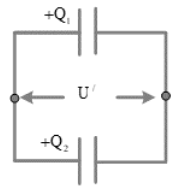
\includegraphics{../figs/VN11-2021-PH-TP007-1}
			\end{center}
		\end{minipage}
	}
	
	\loigiai{
	Điện tích được bảo toàn nên:	
		$$Q=Q' \Rightarrow (C_1 + C_2) U' = C_1 U \Rightarrow U' = \dfrac{U}{1+\dfrac{C_2}{C_1}} = \SI{200}{V}.$$
		
		Tìm được $Q_1=C_1U' = \SI{4e-3}{C}$; $Q_2=C_2U'=\SI{2e-3}{C}$.
	}
	\item \mkstar{4}
	
	\cauhoi{
		Một tụ điện phẳng có điện dung $C=\SI{4}{\micro F}$, khoảng cách giữa hai bản tụ là $d=\SI{4}{mm}$, được tích điện đến điện tích $Q=\SI{8e-4}{C}$, các bản tụ đặt song song theo phương thẳng đứng.
		\begin{enumerate}
			\item Tính hiệu điện thế giữa hai bản tụ;
			\item Một quả cầu kim loại có khối lượng $m=\SI{10}{g}$ tích điện $q=\SI{3}{\micro C}$ được treo bằng sợi dây nhẹ, không dãn, cách điện trong không gian giữa hai bản tụ. Xác định góc tạo bởi phương của dây treo và phương thẳng đứng khi quả cầu cân bằng. Lấy $g=\SI{10}{m/s^2}$.
		\end{enumerate}
	}
	
	\loigiai{
		\begin{enumerate}
			\item Tính hiệu điện thế giữa hai bản tụ;
			
			$$U=\dfrac{Q}{C} = \SI{200}{V}.$$
			
			\item Một quả cầu kim loại có khối lượng $m=\SI{10}{g}$ tích điện $q=\SI{3}{\micro C}$ được treo bằng sợi dây nhẹ, không dãn, cách điện trong không gian giữa hai bản tụ. Xác định góc tạo bởi phương của dây treo và phương thẳng đứng khi quả cầu cân bằng. Lấy $g=\SI{10}{m/s^2}$.
			
			Điều kiện cân bằng của quả cầu:
			$$\vec P + \vec F + \vec T = 0.$$
			
			Khi đó:
			$$\tan \alpha = \dfrac{F}{P} = \dfrac{|q|U}{mgd} \Rightarrow \alpha = 56^\circ .$$
		\end{enumerate}
		
	}
	
\end{enumerate}